\chapter{Use case: GSI Bot}
\label{chap:usecasegsi}

\begin{chapterintro}

In this chapter, we will describe the prototype we developed for a bot for the GSI web page following the architecture described in chapter \ref{chap:architecture}. We will start with the process to recover the data as Linked Data, to them describe the interface and the modules of the system.
 
\end{chapterintro}

\cleardoublepage

\section{Overview of the system}

Along with the prototype described in chapter \ref{chap:usecasejava}, we have also developed a system with the data from the GSI webpage, including data from the projects, publications and staff. For this, we have similar modules:

\begin{enumerate}
 \item A Javascript client acting as the user interface.
 \item A Python controller, handling the flow of the information in the system
 \item A different ChatScript bot, handling the conversation.
 \item An Apache Solr core, with all the data.
\end{enumerate}

In this case, the data was recovered using a mix of techniques, and integrated into a single core in Solr.

\section{Recovering and storing the data}

Similarly to the previous chapter, the data for this prototype has been recovered and converted into RDF and json formats, 

\subsection{Webpage categories}

We considered three types of data from the GSI web page: the information about the members of the groups, their publications and the projects the groups has taken part of. Each type comes from a different part of the website, and therefore will be considered independently. 

\subsubsection{Projects}

For the projects information, the data is available in different formats in the webpage itself, including RDF/XML, as shown in figure \ref{fig:gsiprojects}

\begin{figure}[!htbp]
    \centering
    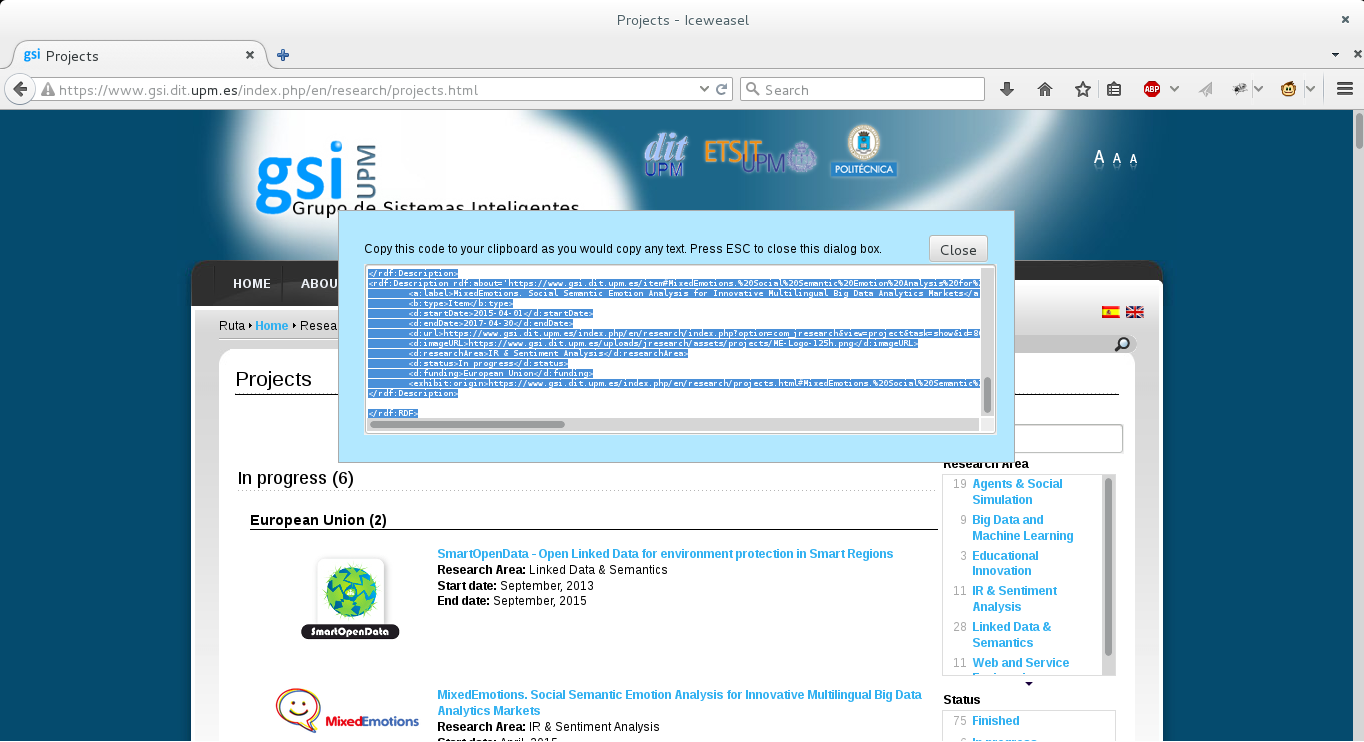
\includegraphics[width=0.8\textwidth]{img/screens/gsi-projects.png}
    \caption{RDF exporter for the projects.}
    \label{fig:gsiprojects}
\end{figure}


\subsubsection{Publications}

Each publication listed in the GSI webpage has an attached bibtex citation. Therefore, using a bibtex ontology\footnote{\url{http://purl.oclc.org/NET/nknouf/ns/bibtex}} to map the elements in the bibtex files to semantic data.  The mapping for the classes is shown in table \ref{tab:bibtex-classes}. As with the classes, the mapping of the properties is very straightforward, and therefore we will not go into details here

\begin{center}
  \begin{table}
    \begin{tabular*}{0.7\textwidth}{@{\extracolsep{\fill}} | c | c | p{0.5\textwidth} |}
      \hhline{|-|-|-|}
      \textbf{Bibtex tag} & \textbf{Ontolgoy mapping} & \textbf{Description} \\ \hhline{|=|=|=|}
      article & bibtex:Article & An article from a journal or magazine. \\ \hhline{|-|-|-|}
      book & bibtex:Book & A book with an explicit publisher. \\ \hhline{|-|-|-|}
      conference & bibtex:Conference & An article in a conference proceedings. \\ \hhline{|-|-|-|}
      inbook & bibtex:Inbook & A part of a book, which may be a chapter (or section or whatever) and/or a range of pages. \\ \hhline{|-|-|-|}
      onCollection & bibtex:Incollection & A part of a book having its own title. \\ \hhline{|-|-|-|}
      masterthesis & bibtex:Masterthesis & A Master's thesis \\ \hhline{|-|-|-|}
      phdthesis & bibtex:Phdthesis & A PhD thesis. \\ \hhline{|-|-|-|}
      proceedings & bibtex:Proceedings & The proceedings of a conference \\ \hhline{|-|-|-|}
      techreport & bibtex:Techreport & A report published by a school or other institution, usually numbered within a series. \\ \hhline{|-|-|-|}
      \end{tabular*}
    \caption{Classes for the bibtex documents.}
    \label{tab:bibtex-classes}
  \end{table}
\end{center}



\subsubsection{People}

\emph{\textcolor{red}{Using Scrappy}}

\subsection{Merging the data}

\section{User interface}


In our prototype, the interaction with the system is done via a web client that provides a chat box and an iframe where the content is located. When the user first opens the page, it's greeted by the bot, and provided with a   short explanation of how the client works.

\begin{figure}[!htbp]
    \centering
    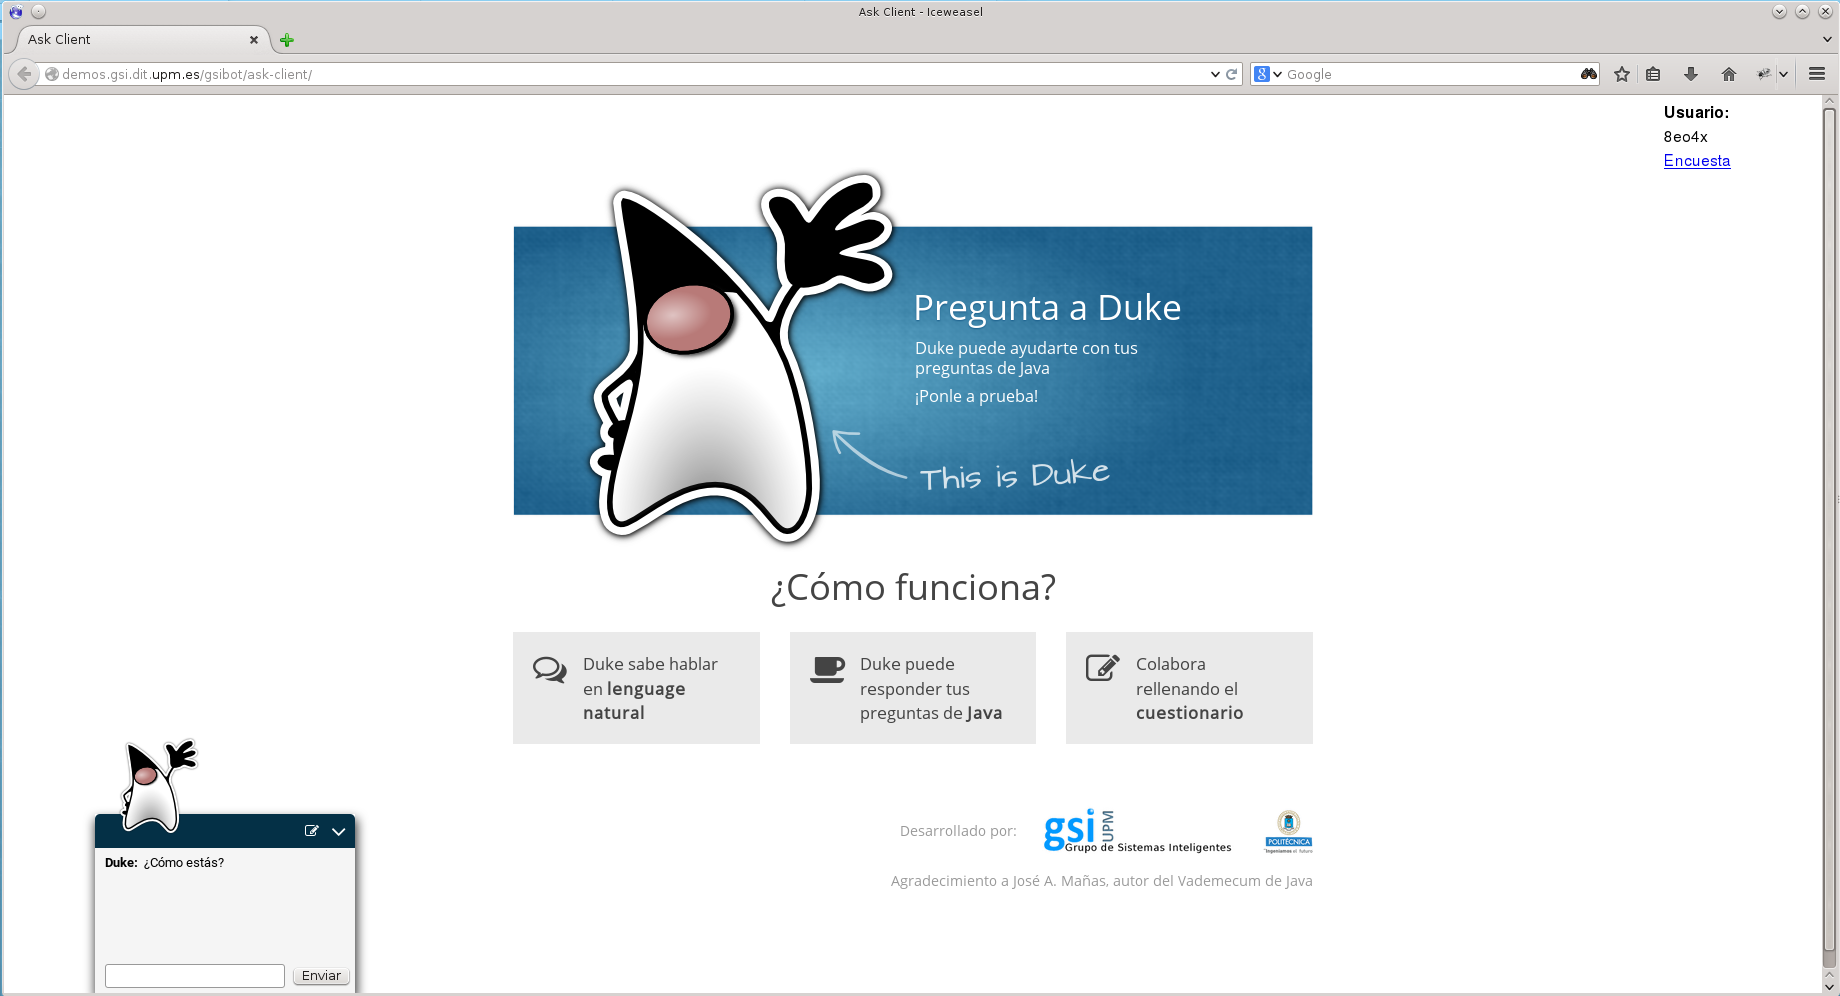
\includegraphics[width=0.7\textwidth]{img/screens/ask-client.png}
    \caption{Web interface for the client.}
    \label{fig:chat1}
\end{figure}

The client is made using web technologies: HTML, CSS and Javascript, and uses Ajax to communicate with the server sending the user questions and handling the response, waiting for the user to send a question and then making the request to the server, as shown in listing \ref{listing:formclient}.

%\emph{\textcolor{red}{Add example of JSON request? Add html code?}}

\begin{center}
  \lstinputlisting[language=JavaScript, caption=Ajax performing the request to the controller, label=listing:formclient, firstline=77, lastline=118]{code/prot/ask.js}
\end{center}

Upon the user submitting a question through the interface, the client will send a GET request to the controller, as described in section~\ref{sec:frontendcon}, and will receive a json response, containing the answer and the page to be shown to the user, if existent. An example response to que question ``¿Qué es un for?'' is shown in listing~\ref{listing:jsonchatresponse}.

\begin{center} 
  \begin{lstlisting}[language=json, caption=Example response for the chat client, label=listing:jsonchatresponse]
   {
     "answer": [
		"Esto es lo que s\u00e9 sobre for",
		"Si quieres, creo que bucles for degenerados tienen algo que ver con esto"
	       ],
     "definition": "Los bucles for se ejecutan un n\u00famero determinado de veces",
     "links": [
                "http://www.dit.upm.es/~pepe/libros/vademecum/topics/3.html",
                "http://www.dit.upm.es/~pepe/libros/vademecum/topics/139.html",
                "http://www.dit.upm.es/~pepe/libros/vademecum/topics/140.html",
                "http://www.dit.upm.es/~pepe/libros/vademecum/topics/141.html",
                "http://www.dit.upm.es/~pepe/libros/vademecum/topics/142.html",
                "http://www.dit.upm.es/~pepe/libros/vademecum/topics/143.html"
                ] ,
     "resource": "http://www.dit.upm.es/~pepe/libros/vademecum/topics/138.html"
   }  
  \end{lstlisting}
\end{center}


\section{Controller}



\section{Chatbot}

\subsection{Rules}

\section{Solr instance}

\subsection{Solr Schema}

\subsection{Solr queries}
